\documentclass[fontsize = 10pt, paper= a4,twocolumn,column_gap=5zw]{jlreq}

\usepackage[dvipdfmx]{graphicx}
\usepackage{color}
\usepackage{listings}
\usepackage{url}
\definecolor{OliveGreen}{rgb}{0.0,0.6,0.0}
\definecolor{Magenta}{cmyk}{0, 1, 0, 0}
\definecolor{colFunc}{rgb}{1,0.07,0.54}
\definecolor{CadetBlue}{cmyk}{0.62,0.57,0.23,0}
\definecolor{Brown}{cmyk}{0,0.81,1,0.60}
\definecolor{colID}{rgb}{0.63,0.44,0}
\lstset{
language={C},                   %言語の指定
basicstyle={\ttfamily\small},        %書体の指定
backgroundcolor={\color[gray]{.95}}, %背景色と透過度
keywordstyle={\color{blue}},         %キーワード(int, ifなど)の書体指定
commentstyle={\color{OliveGreen}},   %注釈の書体 
stringstyle=\color{Magenta},         %文字列
frame=single,                        %枠縁(leftline,topline,bottomline,lines,trBL,shadowbox, single)
numbers=left,                        %行番号表示
numberstyle={\ttfamily\small},       %行番号の書体指定
breaklines=true,                     %折り返し(自動改行)
breakindent = 10pt,                  %自動改行後のインデント量(デフォルトでは20[pt])	
tabsize=2,                           %タブの大きさ
captionpos=t                         %キャプションの場所(t,b : "tb"ならば上下両方に記載)
}
\renewcommand{\lstlistingname}{図} % キャプション名の指定

\begin{document}

\title{統計分析法 第二週レポート}
\author{202212022 田島瑞起}
\date{2023/10/15}
\maketitle
\section{設問0}
(平均値) = $99.93515$
グラフは,下記の通りとなった。
\begin{figure}
    \centering
    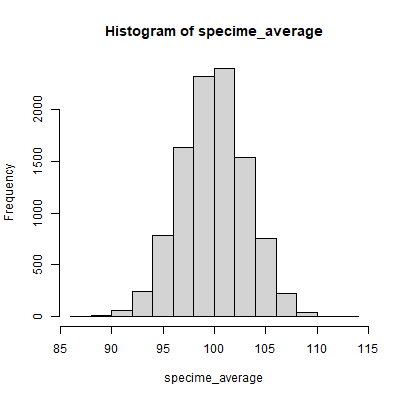
\includegraphics[width=5cm]{kadai0.png}
\end{figure}

\section{設問2}
(平均値) = $71.18$,(不偏標本標準偏差) =  =$13.11165$

\section{設問3}
図は下記の通りとなった。
\begin{figure}
    \centering
    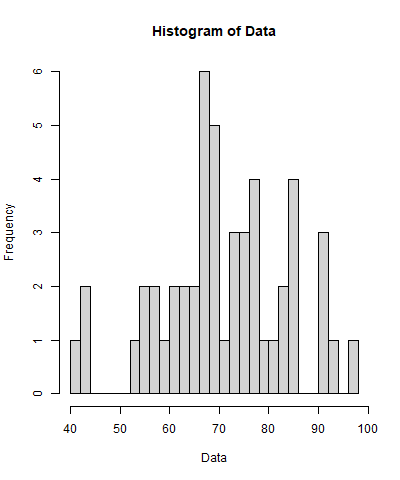
\includegraphics[width=5cm]{kadai3.png}
\end{figure}

\section{設問4}
5個のサンプルデータにおける平均値は58.2,標準誤差は8.077128
10個のサンプルデータにおける平均値は67.2,標準誤差は6.17306
20個のサンプルデータにおける平均値は68.85,標準誤差は3.51259

\section{設問6}
(平均値) = $99.93515$
グラフは,下記の通りとなった。
\begin{figure}
    \centering
    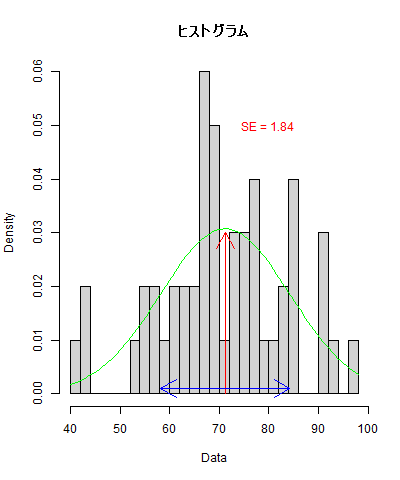
\includegraphics[width=4cm]{kadai5.png}
\end{figure}

\section{ソースコード}
\begin{lstlisting}[basicstyle=\ttfamily\footnotesize, frame=single, caption=s2212022-1.c ,label=s2212022-1.c]
    #課題1.
    #仮説検定とt検定によって執り行う
    #H_0はAとBに差がない
    #H_1はAとBに差がないとは言えない(A-Bの値が優位水準を満たさない)
    Data <- read.table("weight.txt",header=TRUE)
    t.test(Data$A,Data$B,paired=TRUE,var.equal=TRUE)
    
    #課題2.
    #平均値と標準偏差を求める
    Mean_A <- mean(Data$A)
    Mean_B <- mean(Data$B)
    Mean_A 
    Mean_B
    SD_A <- sd(Data$A)
    SD_B <- sd(Data$B)
    SD_A
    SD_B
    
    png("3-2-1.png", width = 400, height = 400)
    hist(Data$A,freq=FALSE)
     # 矢印を描画
    arrows(x0 = Mean_A,  y0 = 0.025, x1 = Mean_A, y1 = 0, col = "red", code = 1, angle = 30)
    arrows(x0 = Mean_A + SD_A , y0 = 0.014, x1 = Mean_A, y1 = 0.014, col = "blue", code = 1, angle = 30)
    arrows(x0 = Mean_A - SD_A,  y0 = 0.014, x1 = Mean_A, y1 = 0.014, col = "blue", code = 1, angle = 30)
    # 正規分布で近似した曲線を追加
    x <- seq(min(Data$A), max(Data$A), length = 100)
    y <- dnorm(x, mean = Mean_A, sd = SD_A)
    lines(x, y, col = "green")
    text(80,0.030,labels = paste("Mean_A =", round(Mean_A, 2)), col = "red")
    text(80,0.025,labels = paste("SD_A =", round(SD_A, 2)), col = "red")
    dev.off()
    
    
    
    png("3-2-2.png", width = 400, height = 400)
    hist(Data$B,freq=FALSE)
     # 矢印を描画
    arrows(x0 = Mean_B,  y0 = 0.025, x1 = Mean_B, y1 = 0, col = "red", code = 1, angle = 30)
    arrows(x0 = Mean_B + SD_B , y0 = 0.014, x1 = Mean_B, y1 = 0.014, col = "blue", code = 1, angle = 30)
    arrows(x0 = Mean_B - SD_B,  y0 = 0.014, x1 = Mean_B, y1 = 0.014, col = "blue", code = 1, angle = 30)
    # 正規分布で近似した曲線を追加
    x <- seq(min(Data$B), max(Data$B), length = 100)
    y <- dnorm(x, mean = Mean_B, sd = SD_B)
    lines(x, y, col = "green")
    text(80,0.025,labels = paste("Mean_B =", round(Mean_B, 2)), col = "red")
    text(80,0.020,labels = paste("SD_B =", round(SD_B, 2)), col = "red")
    dev.off()
    
    
    #課題3.
    #p = 2.8*10^(-2)より優位水準を満たさないのでH_0は棄却される
    # 自由度は49
    #帰
    
    #課題4
    #H_0は棄却され,AとBのデータセットには差があるということがわかる。
    
    #課題5
    Data <- read.table("weight.txt",header=TRUE)
    t.test(Data$A,Data$B,paired=FALSE,var.equal=TRUE)
    #関連2群t-検定では同一集団の条件比較がなされるのに対して,独立2群t-検定では独立した集団のデータに差異があるかどうか示すものであるため,違いが生まれるといって良い
    
    #課題6
    #t-検定を行う条件として分散が少ないことが必要である
    #⓵与えられたそれぞれのデータが正規分布に近いということ⓶与えられたそれぞれのデータの分散がほぼ等しいこと    
    \end{lstlisting}

\end{document}